\documentclass[../../presentazione_orale.tex]{subfiles}

\onlyinsubfile{\author{Matteo Zortea, Elena Acinapura}
\title{Esperienza di Faraday}
\date{Settembre 2020}}

\begin{document}

\onlyinsubfile{\maketitle}

Valori dei componenti rilevanti:
\begin{itemize}
    \item $R_{lim} = 10.184\pm0.002 \si{\ohm}$
    \item numero avvolgimenti bobine: $n_1 = 28$, $n_2 = 30$
    \item frequenze usate: $1\si{\kilo\hertz}$, $50\si{\kilo\hertz}$, $150\si{\kilo\hertz}$
\end{itemize}

\begin{figure}[h!]
    \centering
    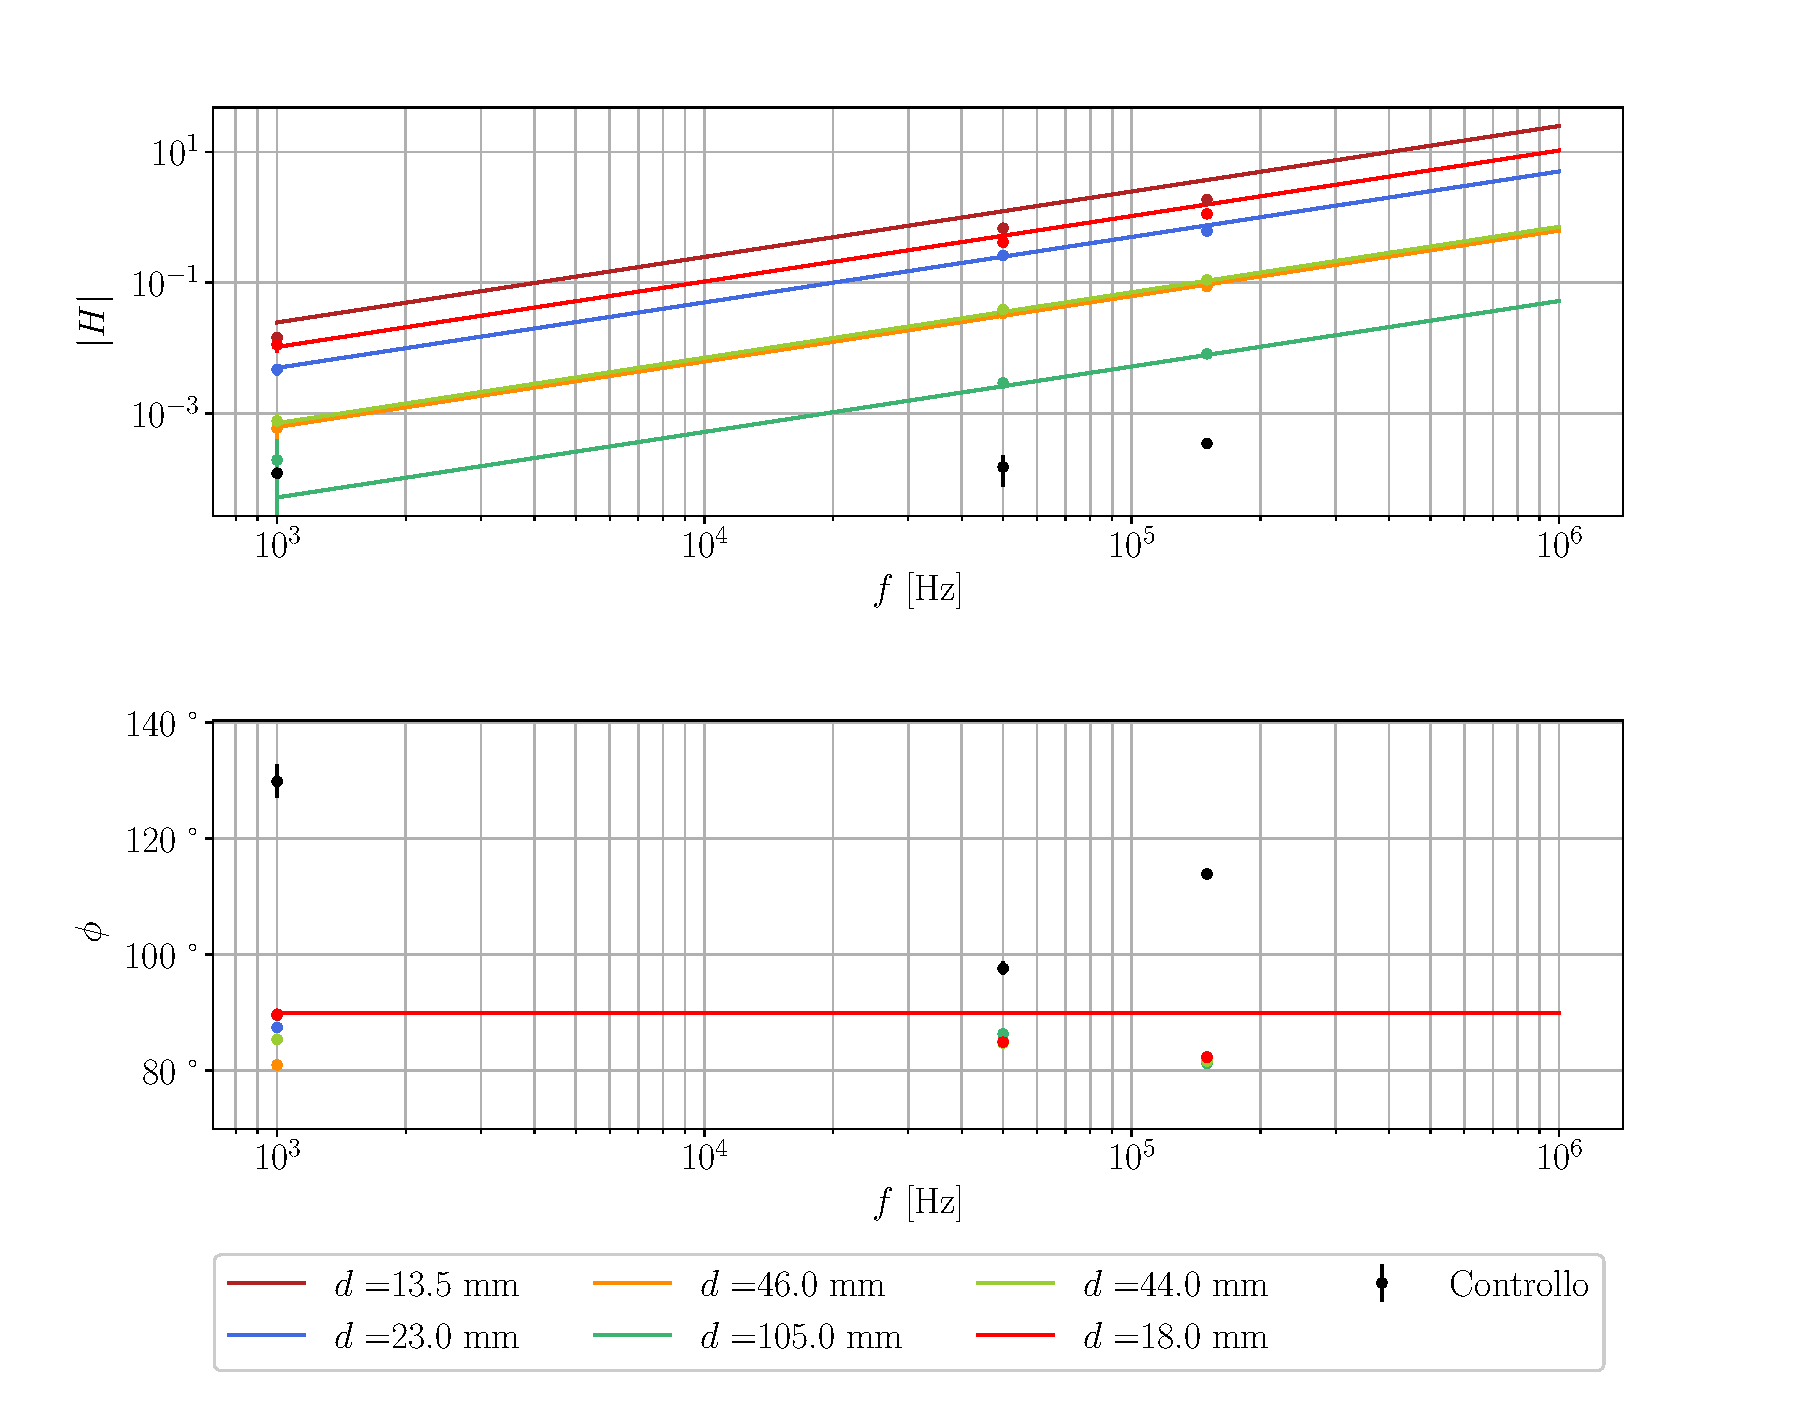
\includegraphics[scale = 0.55]{Grafici/bode.eps}
    \caption{\textbf{Bodeplot} di $Z_{eff}$ in funzione della frequenza per diverse $d$.}
    \label{fig:bode}
\end{figure}

\begin{figure}[h!]
    \centering
    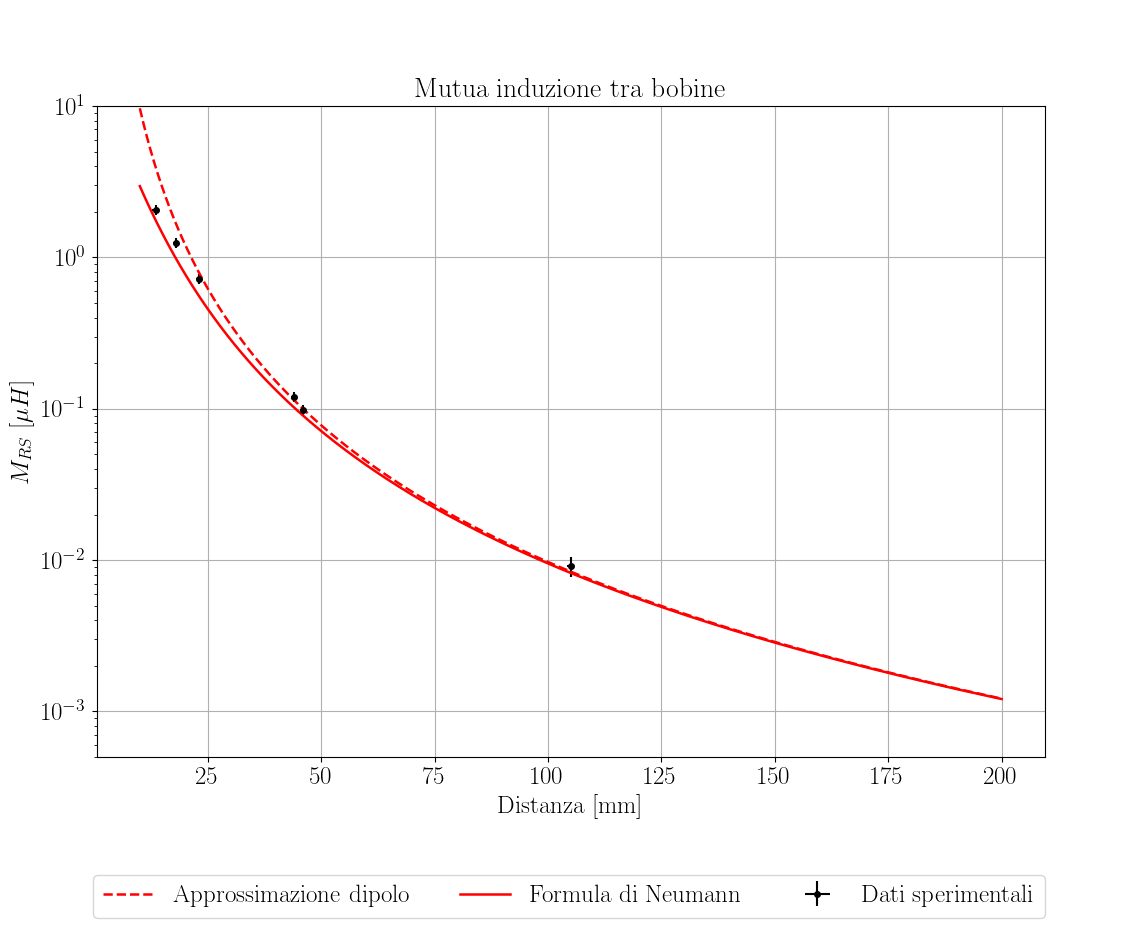
\includegraphics[scale = 0.55]{Grafici/induttanza2.png}
    \caption{Mutua induzione tra bobine, $M_{RS}$, in funzione della distanza tra le bobine stesse.}
    \label{fig:induzione}
\end{figure}
Stima dell'accoppiamento tra i circuiti in assenza di bobine:
$$ Z_{ctrl} = 0.33\pm0.11~\si{\nano\henry}$$
\end{document}